\documentclass{article}

\usepackage{graphicx}
\usepackage{tikz}
\usepackage{tikzsymbols}
\usetikzlibrary{calc,patterns,shapes.geometric}
\pagestyle{empty}
\usepackage[margin=0pt]{geometry}
\geometry{papersize={14in,12in}}

\def\centerarc[#1](#2)(#3:#4:#5){\draw[#1] ($(#2)+({#5*cos(#3)},{#5*sin(#3)})$) arc (#3:#4:#5);}

\begin{document}
	\begin{figure}
		\centering
		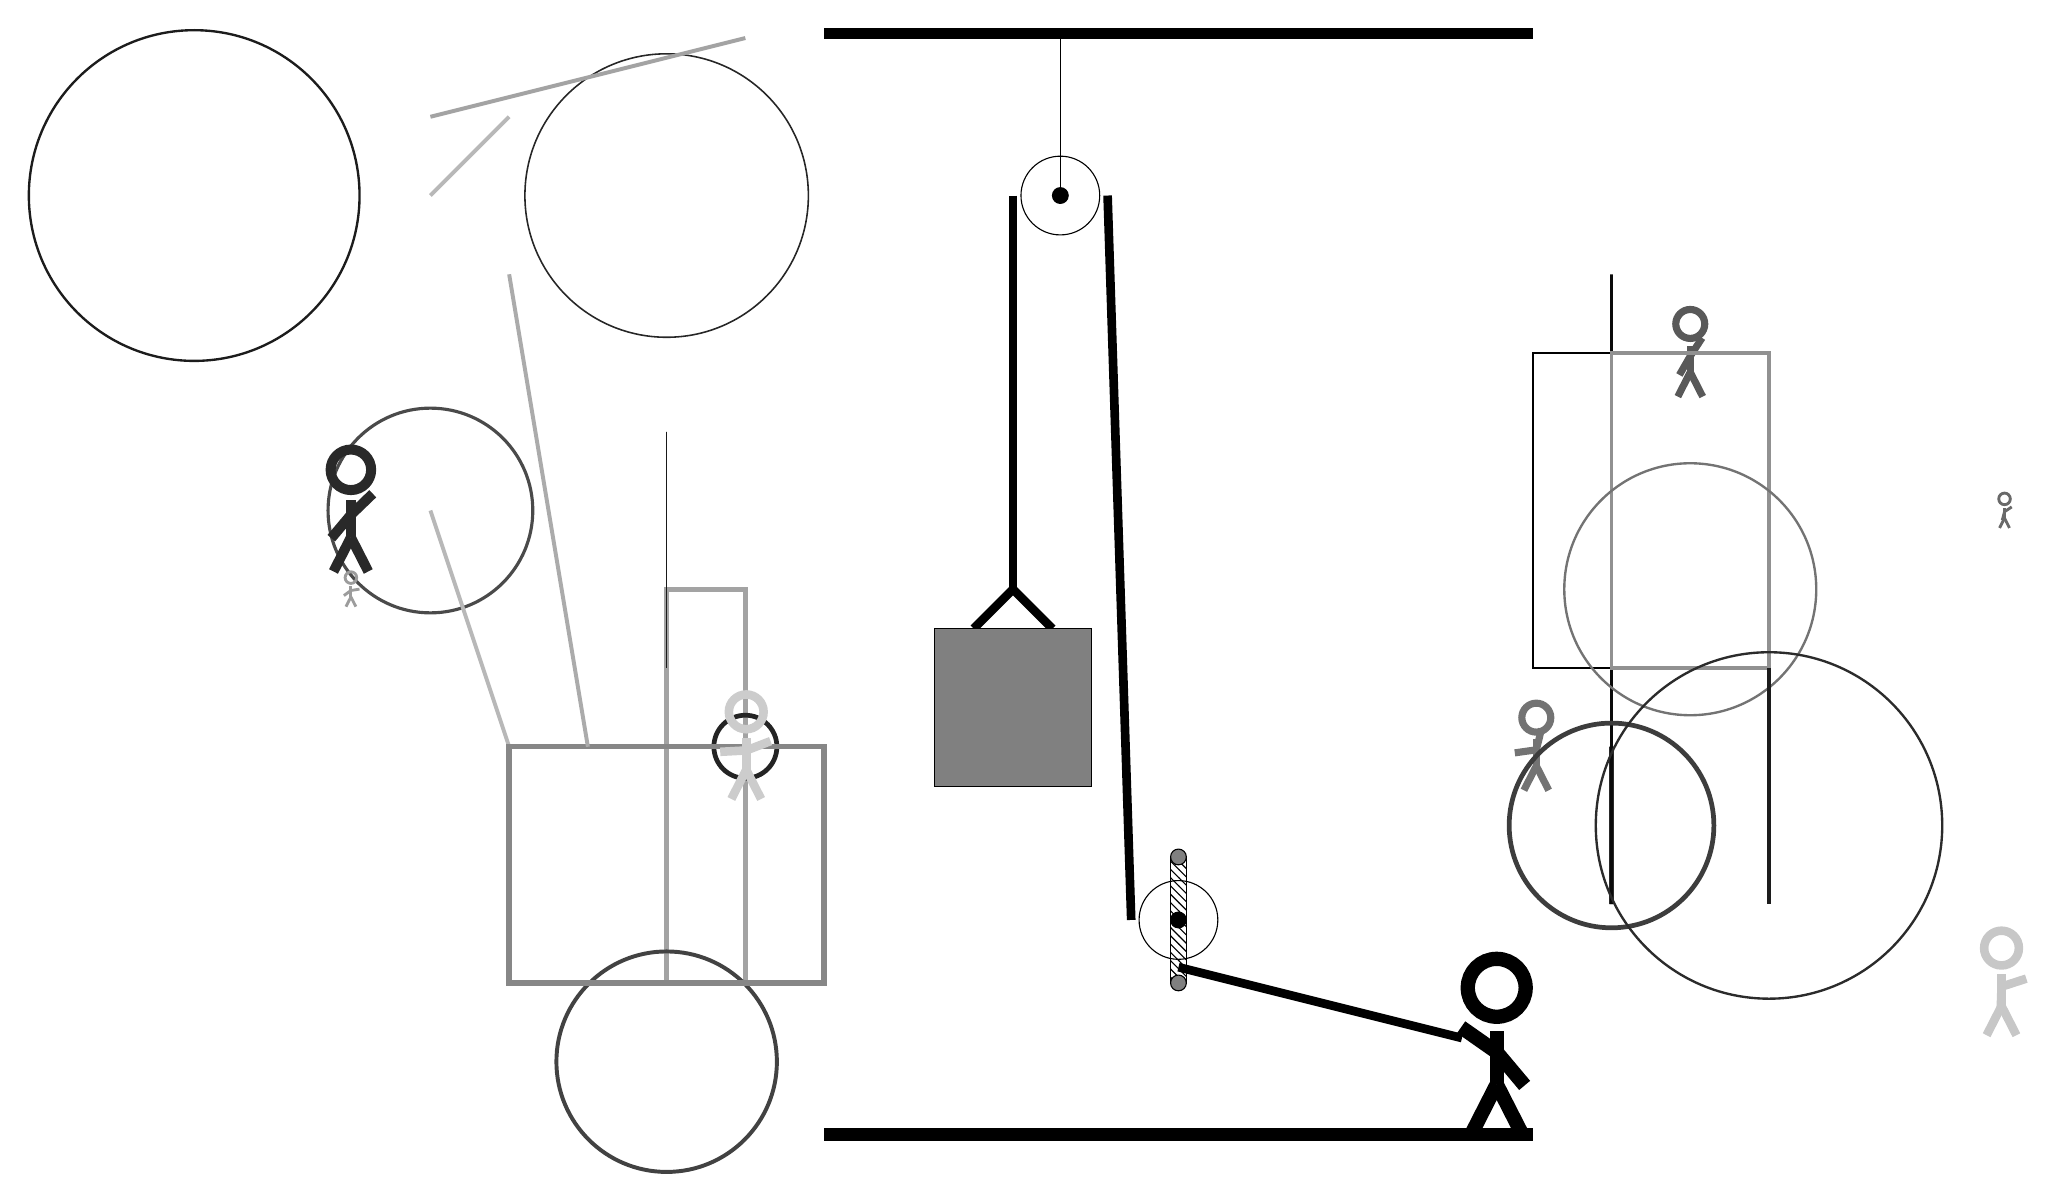
\begin{tikzpicture}
			%%%%% START %%%%%
			
			\draw[fill=black] (-2, 14) rectangle (7, 14.125);
			
			\draw[line width=0.7mm, color=black!84] (8, 5) rectangle (8, 3);
			
			\node[line width=0.6mm, color=black!55] at (7, 5) {\Strichmaxerl[5][8][76]};
			\draw [line width=0.4mm, color=black!71](-7, 8) circle (1.3);
			\node[line width=0.4mm, color=black!39] at (-8, 7) {\Strichmaxerl[2][36][9]};
			\draw[line width=0.3mm, color=black!100] (8, 6) rectangle (7, 10);
			\draw[line width=0.6mm, color=black!36] (-4, 2) rectangle (-3, 7);
			\draw [line width=0.3mm, color=black!89](-10, 12) circle (2.1);
			
			\node[line width=0.3mm, color=black!65] at (9, 10) {\Strichmaxerl[5][60][57]};
			\draw [line width=0.2mm, color=black!85](-4, 12) circle (1.8);
			\node[line width=0.7mm, color=black!22] at (13, 2) {\Strichmaxerl[6][88][18]};
			\draw[line width=0.5mm, color=black!28](-6, 5) -- (-7, 8);
			
			\draw[line width=0.4mm, color=black!96] (8, 3) rectangle (8, 11);
			\draw[line width=0.4mm, color=black!43] (8, 10) rectangle (10, 6);
			
			\node[line width=0.3mm, color=black!59] at (13, 8) {\Strichmaxerl[2][75][34]};
			\draw[line width=0.5mm, color=black!28](-7, 12) -- (-6, 13);
			\draw [line width=0.3mm, color=black!55](9, 7) circle (1.6);
			
			\draw [line width=0.5mm, color=black!74](-4, 1) circle (1.4);
			
			\draw[line width=0.5mm, color=black!36](-7, 13) -- (-3, 14);
			\draw[line width=0.5mm, color=black!89](10, 6) -- (10, 3);
			\node[line width=0.5mm, color=black!84] at (-8, 8) {\Strichmaxerl[7][50][44]};
			\draw [line width=0.6mm, color=black!76](8, 4) circle (1.3);
			\draw [line width=0.6mm, color=black!86](-3, 5) circle (0.4);
			\draw[line width=0.7mm, color=black!47] (-2, 2) rectangle (-6, 5);
			\draw [line width=0.3mm, color=black!83](10, 4) circle (2.2);
			\node[line width=0.3mm, color=black!20] at (-3, 5) {\Strichmaxerl[6][3][21]};
			
			\draw[line width=0.2mm, color=black!90] (-4, 9) rectangle (-4, 6);
			
			\draw[line width=0.5mm, color=black!33](-6, 11) -- (-5, 5);
			
			\draw (1, 12) circle (0.5);
			\draw[fill=black] (1, 12) circle (0.1);
			\draw (1, 14) -- (1, 12);
			
			\draw[fill=white](2.5, 2.8) circle (0.5);
			\draw[fill=black] (2.5, 2.8) circle (0.1);
			\draw[pattern=north west lines, pattern color=black] (2.4, 3.6) rectangle (2.6, 2.0);
			\draw[fill=black!50] (2.5, 3.6) circle (0.1);
			\draw[fill=black!50] (2.5, 2.0) circle (0.1);
			
			\draw[line width=1.1mm] (-0.1, 6.5) -- (0.4, 7.0) -- (0.9, 6.5);
			\draw[fill=black!50] (-0.6, 6.5) rectangle (1.4, 4.5);
			
			\draw[line width=1.1mm] (0.4, 12) -- (0.4, 7.0);
			\centerarc[line width=1.1mm](1, 12)(0:180:0.6);
			\draw[line width=1.1mm](1.6, 12) -- (1.9, 2.8);
			\centerarc[line width=1.1mm](2.5, 2.8)(180:270:0.6);
			\draw[line width=1.1mm](2.5, 2.2) -- (6.1, 1.3);
			
			\node at (6.5, 1.2) {\Strichmaxerl[10][-35][-50]};
			
			\draw[fill=black] (-2, 0) rectangle (7, 0.15);
			
			%%%%% END %%%%%
		\end{tikzpicture}
	\end{figure}	
\end{document}